\documentclass[9pt]{beamer}
\usepackage[utf8]{inputenc}
\usepackage{enumitem}
\usepackage{graphicx}
\usepackage{array}
\usepackage{mdwlist}
\usepackage{floatrow}
\usepackage{hyperref}
\usepackage{listings}
\usepackage{color}
\usepackage{nameref}
\usepackage{algorithm}
\usepackage{algorithmic}

\graphicspath{ {img/}, {../RASD/img/} }

\makeatletter
\newcommand*{\currentname}{\@currentlabelname}
\makeatother

\newcounter{saveenumi}
\newcommand{\seti}{\setcounter{saveenumi}{\value{enumi}}}
\newcommand{\conti}{\setcounter{enumi}{\value{saveenumi}}}

\usetheme{Warsaw}

\AtBeginSection[]
{
  \begin{frame}
    \frametitle{Table of Contents}
		\setcounter{tocdepth}{2}
    \tableofcontents[currentsection]
  \end{frame}
}

\title{myTaxiService}
\subtitle{Design Document}
\author{Jacopo Strada, Luca Riva}
\date{December 9, 2015}

\begin{document}

\maketitle

\section{Architectural Design}
\subsection{Component View}
\begin{frame}{\currentname}

\begin{figure}[H]
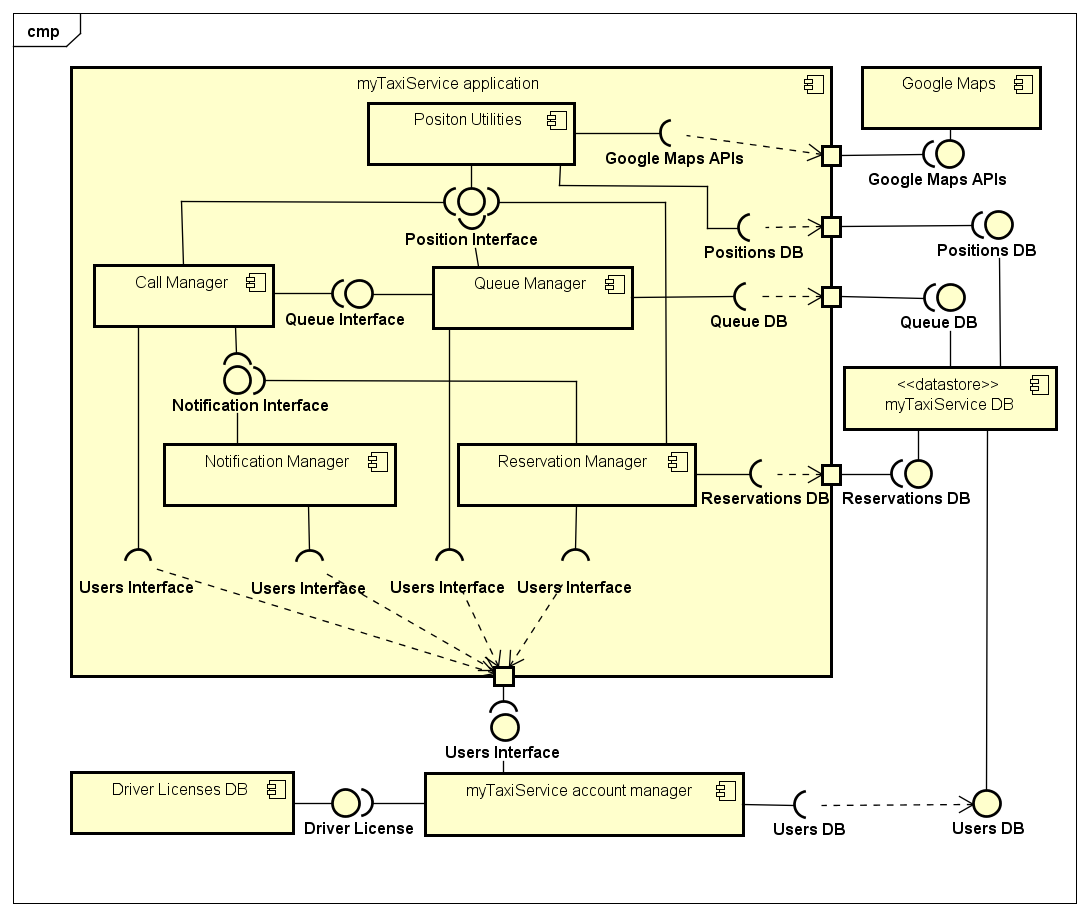
\includegraphics[height=.85\textheight]{ComponentDiagram}
\centering
\end{figure}

\end{frame}

\subsection{Deployment View}
\begin{frame}{\currentname}

\begin{figure}[H]
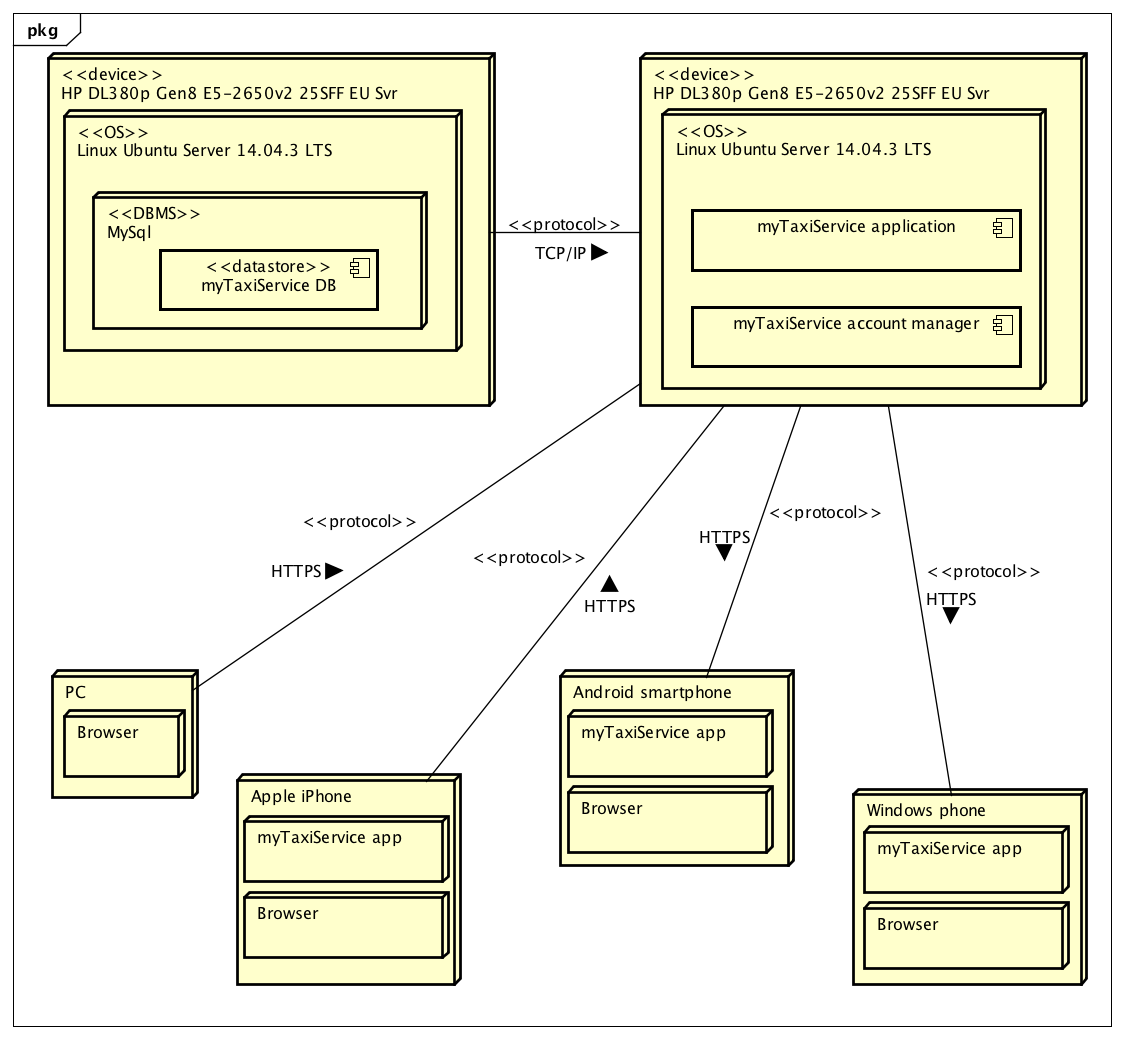
\includegraphics[height=.85\textheight]{DeploymentDiagram}
\centering
\end{figure}

\end{frame}

\subsection{Component Interfaces}
\begin{frame}[allowframebreaks]{\currentname}

\begin{description}
\samepage{
\item[Data Base:] (The following methods are not available as APIs but are only private)\
\begin{itemize*}
    \item \textit{createNewClient(email, name, surname, dateOfBirth, phone, password)}
    \item \textit{createNewDriver(email, name, surname, license, phone, password)}
    \item \textit{checkPassword(userId, password)}
    \item \textit{findUserByEMail(email)}
    \item \textit{getDriverState(email)}
    \item \textit{updateDriverState(email, state)}
    \item \textit{getZones()}
    \item \textit{saveRide(origin, destination, date, time)}
    \item \textit{setRideAccepted(rideId, driver)}
    \item \textit{eraseRide(rideId)}
\end{itemize*}}\framebreak \samepage{
\item[Account Manager:]\
\begin{itemize*}
    \item \textit{login(mail, password)}
    \item \textit{registerClient(email, firstName, lastName, telephoneNumber, password)}
    \item \textit{registerDriver(email, firstName, lastName, telephoneNumber, license, password)}
    \item To receive information about an user: \textit{clientInfo(email)} or \textit{drievrInfo(email)}
    \item To change a driver state when they are taking a call: \textit{changeDriverState(email, state)}
\end{itemize*}}\samepage{
\item[Call Manager:]\
\begin{itemize*}
    \item To call a taxi: \textit{forwardCall(email, GPSPosition)}
    \item To show the details of a call (should be used by a driver): \textit{showCallDetails(call)}
\end{itemize*}}\samepage{
\item[Queue Manager:]\
\begin{itemize*}
    \item To retrieve the drivers' queue of a certain zone: \textit{driversQueue(zone)}
\end{itemize*}}\framebreak \samepage{
\item[Reservation Manager:]\
\begin{itemize*}
    \item \textit{newReservation(email, origin, destination, time)}
    \item to show the details of a reservation: \textit{showReservationDetails(reservation)}
\end{itemize*}}\samepage{
\item[Notification Manager:]\
\begin{itemize*}
    \item \textit{sendNotification(list\textless email \textgreater, message)} 
\end{itemize*}}\samepage{
\item[Position Utilities:]\
\begin{itemize*}
    \item to find the zone associated to a given coordinate: \textit{findZone(GPSCoordinate)}
\end{itemize*}}
\end{description}

\end{frame}

\subsection{Selected Architectural Styles and Patterns}
\begin{frame}[allowframebreaks]{\currentname}

\begin{figure}[H]
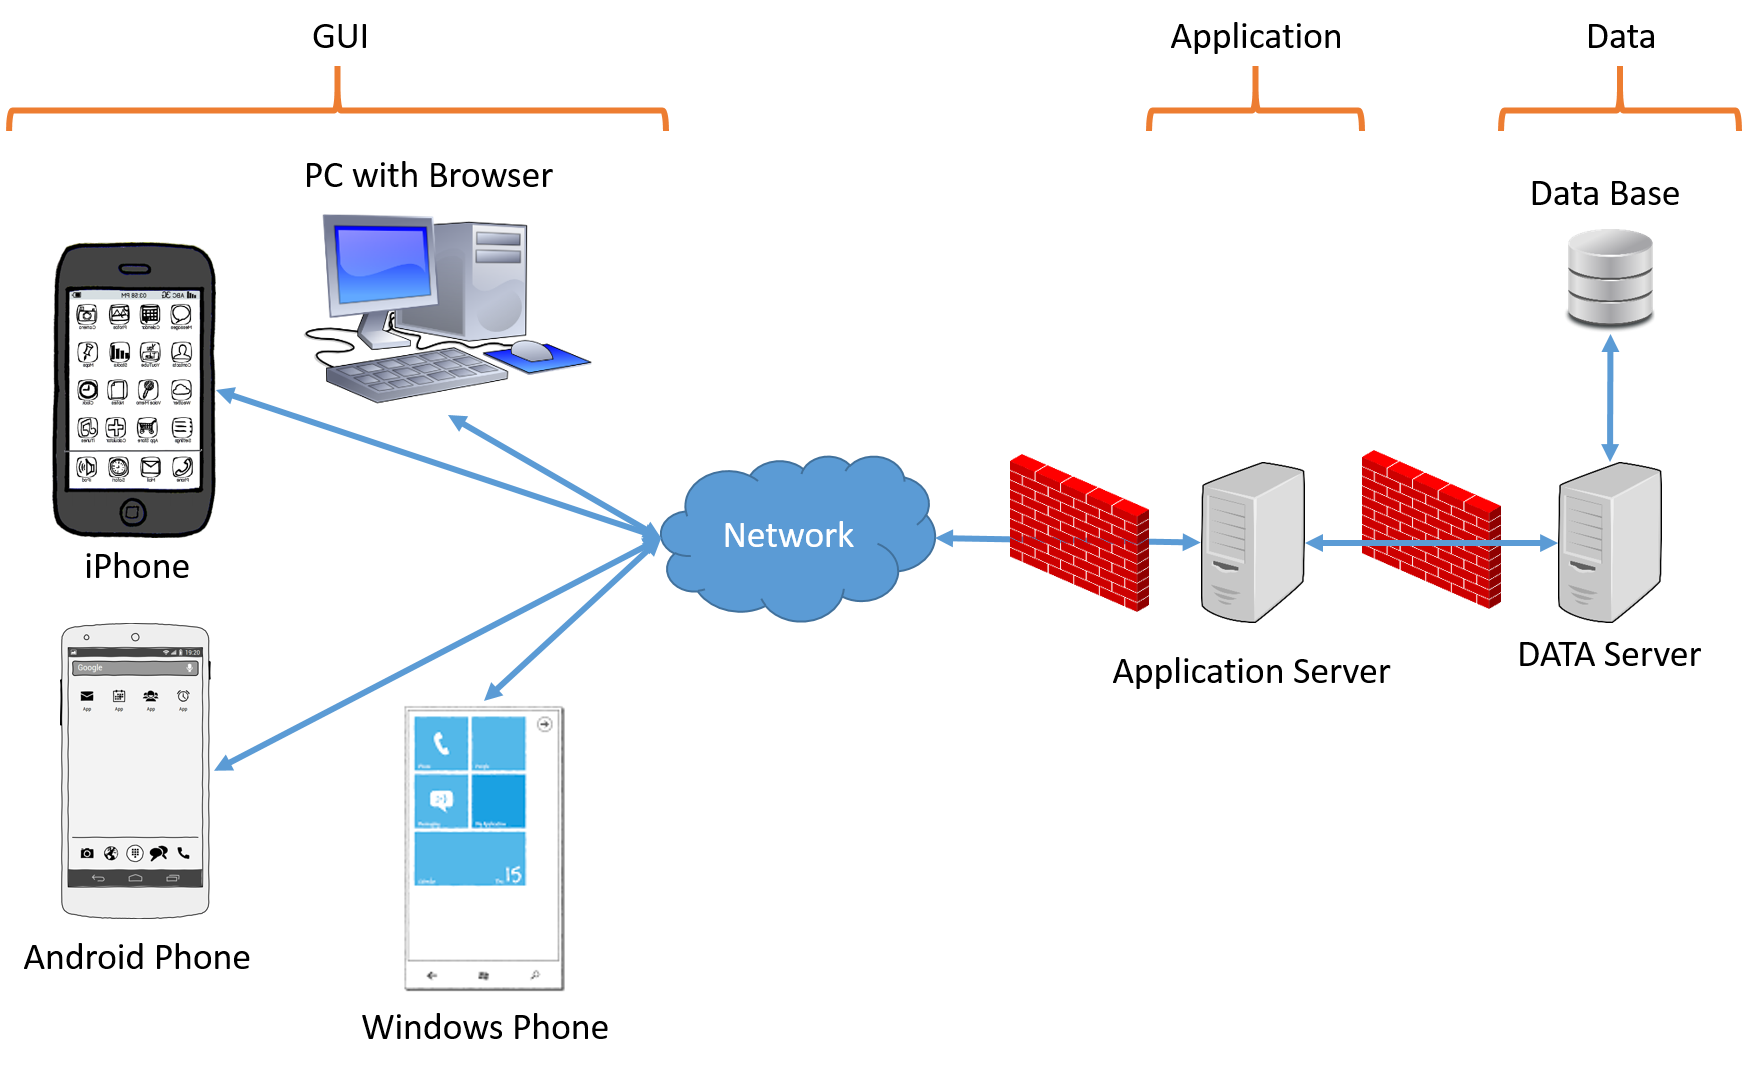
\includegraphics[width=.85\textwidth]{Architecture}
\centering
\end{figure}

\begin{figure}[H]
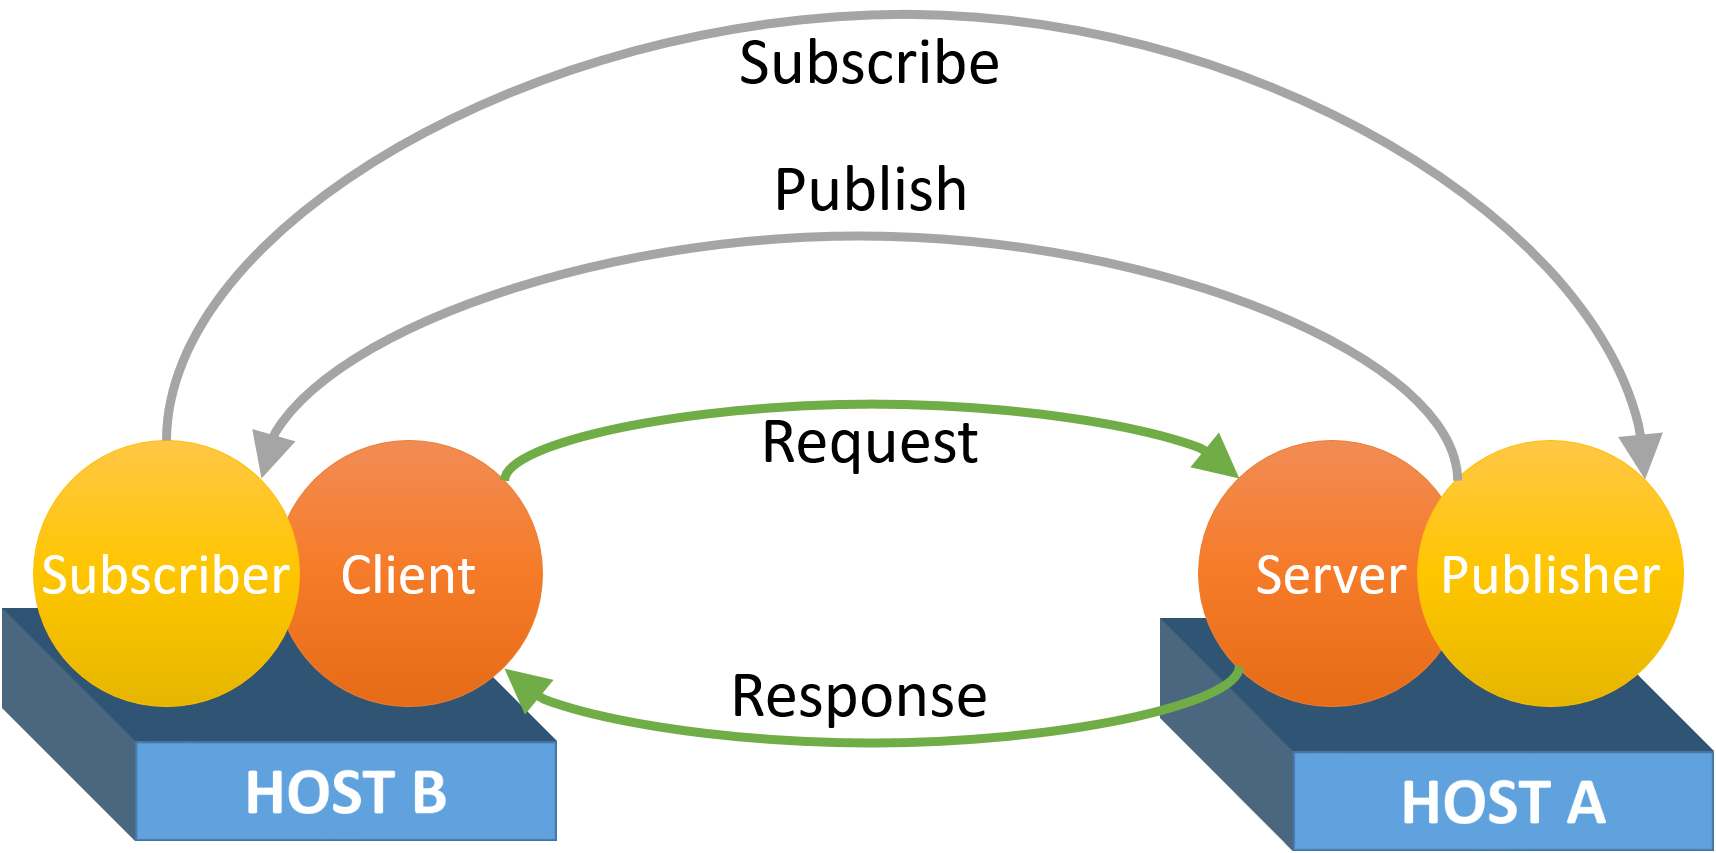
\includegraphics[width=.85\textwidth]{Paradigm}
\centering
\end{figure}

\end{frame}

\section{Algorithm Design}
\begin{frame}{\currentname}

\begin{algorithm}[H]
\algsetup{indent=2em}
\begin{algorithmic}
    
    \REQUIRE the queue of a zone
    \ENSURE the return value is the driver who accepted the ride or NULL if nobody accepted
    
    \FORALL {drivers in queue (only once)}
        \STATE send a notification to the driver
        \STATE wait for 30 seconds (or less if a response is received)
        \IF {the driver has accepted}
            \STATE remove driver from the queue
            \STATE set driver state as \emph{unavailable}
            \STATE send a notification to the client
            \RETURN current driver
        \ELSIF {the driver has rejected \OR the driver hasn't responded}
            \STATE move the driver from the begin to the end of the queue
        \ENDIF
    \ENDFOR
    \RETURN NULL
\end{algorithmic}
\end{algorithm}

\end{frame}

\section{User Interfaces Design}
\subsection{Clients' User Interfaces}
\begin{frame}{\currentname{} - Taxi Call}
\begin{columns}[c]
  \begin{column}{.5\textwidth}
		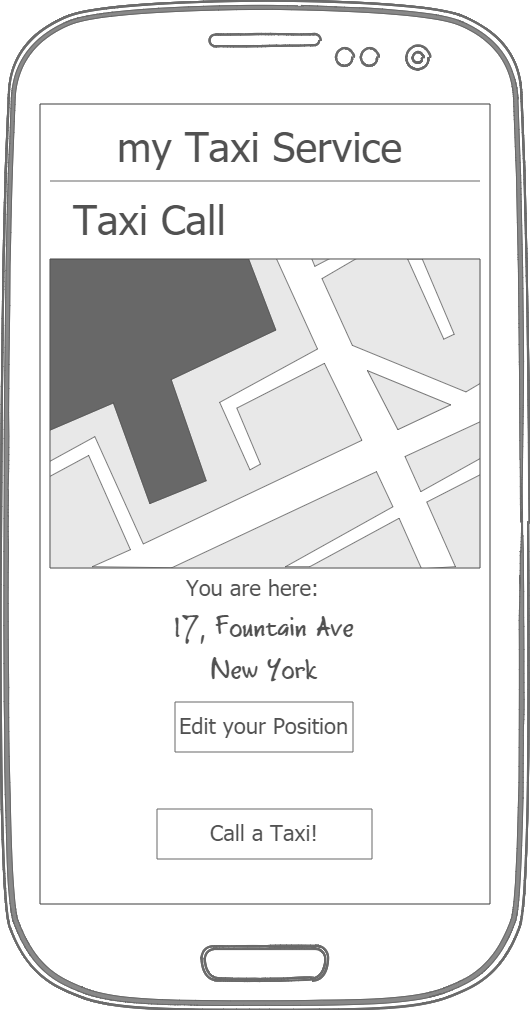
\includegraphics[height=.8\textheight]{Mockup-ClientsTaxiCall}
		\centering
  \end{column}
  \begin{column}{.5\textwidth}
    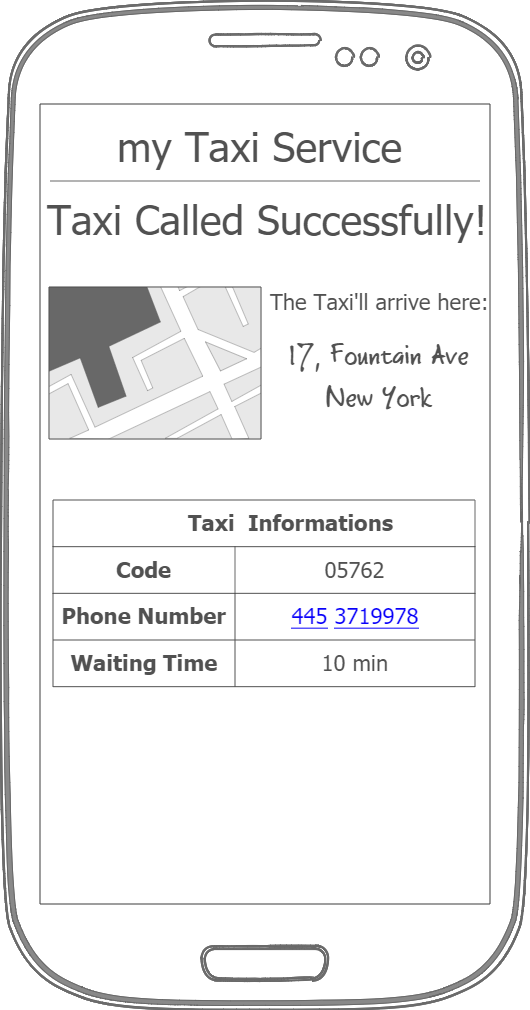
\includegraphics[height=.8\textheight]{Mockup-ClientsTaxiCallConfirmation}
		\centering
  \end{column}
\end{columns}
\end{frame}

\subsection{Taxi Drivers' User Interfaces}
\begin{frame}{\currentname{} - New Requests}
\begin{columns}[c]
  \begin{column}{.5\textwidth}
		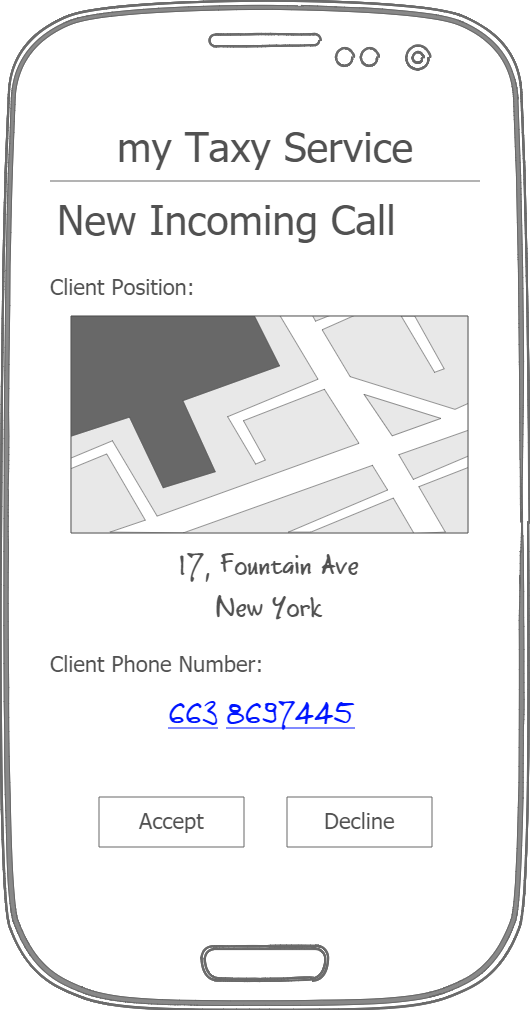
\includegraphics[height=.8\textheight]{Mockup-TaxiDriversNewIncomingCall}
		\centering
  \end{column}
  \begin{column}{.5\textwidth}
    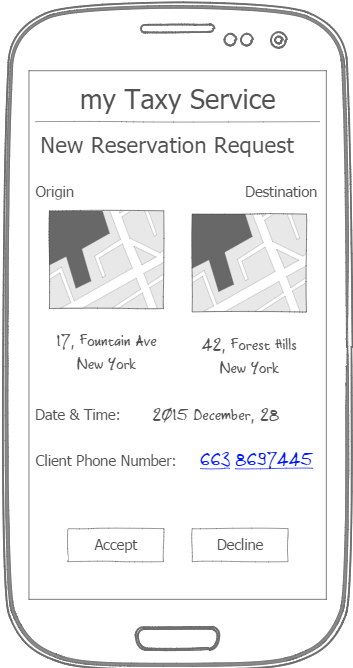
\includegraphics[height=.8\textheight]{Mockup-TaxiDriversReservationRequest}
		\centering
  \end{column}
\end{columns}
\end{frame}

\end{document}